\subsection{Drive-in (limited source diffusion)}
After pre-deposition or ion implant of the initial dosage we need to drive in the ions deeper into the crystal.
In order to prevent back-diffusion into the gas we seal off the oxide window with another layer of oxide in order to make sure that all the dopants stay inside the silicon crystal.

\begin{figure}[H]
	\centering
	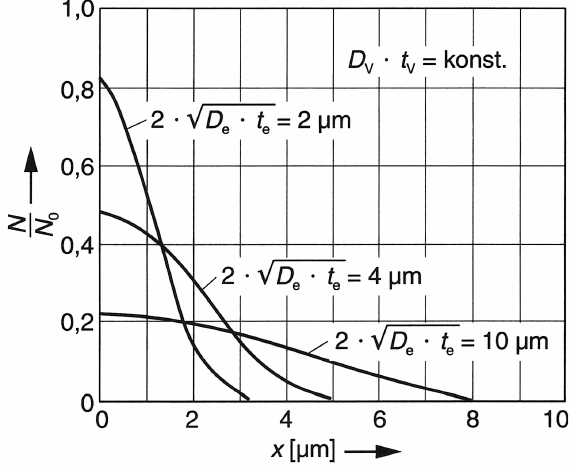
\includegraphics[scale=0.5]{dopants_drive_in_depth.png}
	\caption{Drive-in well depths and concentrations}
\end{figure}

We set the condition that the pre-deposition/implant depth is much lower than the depth of the final diffused volume with the following inequation:
\begin{equation}
x_e = 2 \cdot \sqrt{D_e \cdot t_e} \gg 2 \cdot \sqrt{D_v \cdot t_v} = x_v
\end{equation}
Where $x_v$ is the the depth of the predeposition/implant step.

By neglecting the distribution thickness of the original implantation dosage and assuming that it's comparably thin compared to the medium thickness we can replace  $f(a) \approx \delta(a)$ within \autoref{eq:ficks_law_expanded} which makes
\begin{equation}
N(x,t) = \frac{1}{2 \cdot \sqrt{D} \cdot \sqrt{\pi \cdot t}} \cdot \int_{-\infty}^{\infty}{f(\sqrt{D})\cdot\exp\left(\frac{-(x-\sqrt{D})^2}{4 \cdot D \cdot t^2}\right)}da
\end{equation}
become
\begin{equation}
N(x,t)
=
\frac{1}{2 \cdot \sqrt{D} \cdot \sqrt{\pi \cdot t}} \cdot \int_{-\infty}^{\infty}{\delta(\sqrt{D})\cdot\exp\left(\frac{-(x-\sqrt{D})^2}{4 \cdot D \cdot t^2}\right)}da
\end{equation}
and finally
\begin{equation}
N(x,t)
=
\sqrt{\frac{Q}{\pi \cdot D_e \cdot t}} \cdot \exp\left(\frac{-x^2}{4 \cdot D_e \cdot t^2}\right)
\end{equation}

For a drive-in of boron and phosphorus at $1000\degree C$($1273.15 K$) we can use both $D=2.62 \cdot 10^{-14} \frac{cm^2 }{s}=2.62 \cdot 10^{-18} \frac{m^2 }{s}$
